%!TEX root = ../Main.tex

\chapter{PolyMarker: A fast polyploid primer design pipeline}
%\section{Introduction} 
%Explain how the SNP markers are designed without the tool and an overview. 
One of the main challenges of working with polyploid species is the design of genome specific molecular markers. 
This is particularly true when targeting conserved homoeologue regions, where a primer could bind to a pair,or triplet, of identical sequences. 
For that reason, designing primers for polyploids require to include bases that are specific to the target, in addition to the physicochemical properties of the primer.  
The traditional methodology to find primer candidates include a blast search and a local alignment, select the primer candidates manually, and finally, validate the primers with a tool, like \texttt{Primer3} \citep{Rozen}. 
To reduce the time invested in designed primers I have developed PolyMarker \citep{Ramirez-Gonzalez2015a}, a pipeline to automate the primer design for polyploid organisms.  

\section{Pipeline}
PolyMarker is an automated pipeline that takes as input a list of SNPs and a reference file and produces a list of primer triplets for SNP genotyping. 
The list of SNPs is first converted to a \texttt{FASTA} file with ambiguity codes\citep{Cornish-Bowden1985} 
The sequences are searched on the genomic reference using \texttt{exonerate}\citep{Slater2005} to find the homoeologue regions to the target sequence. 
Then, the alignment between homoeologues is refined using \texttt{MAFFT}\citep{Katoh2013}. 
A list of candidate variations is produced and used as input for \texttt{Primer3}\citep{Rozen}. 
Finally, the output of \texttt{Primer3} is parsed to find the best primer pair that contains a the targeted SNP and a base that is specific to the target genome (Figure \ref{fig:poly:pipeline}).  
The pipeline is written as a Ruby script, using parsers and wrappers from BioRuby \citep{Goto2010} and bio-samtools \citep{Etherington2015,Ramirez-Gonzalez2012}. 
The software is open source and released as a biogem \citep{Bonnal2012}, \texttt{bio-polyploid-tools}, the source code is available in github: \texttt{https://github.com/TGAC/bioruby-polyploid-tools}.

\begin{figure}
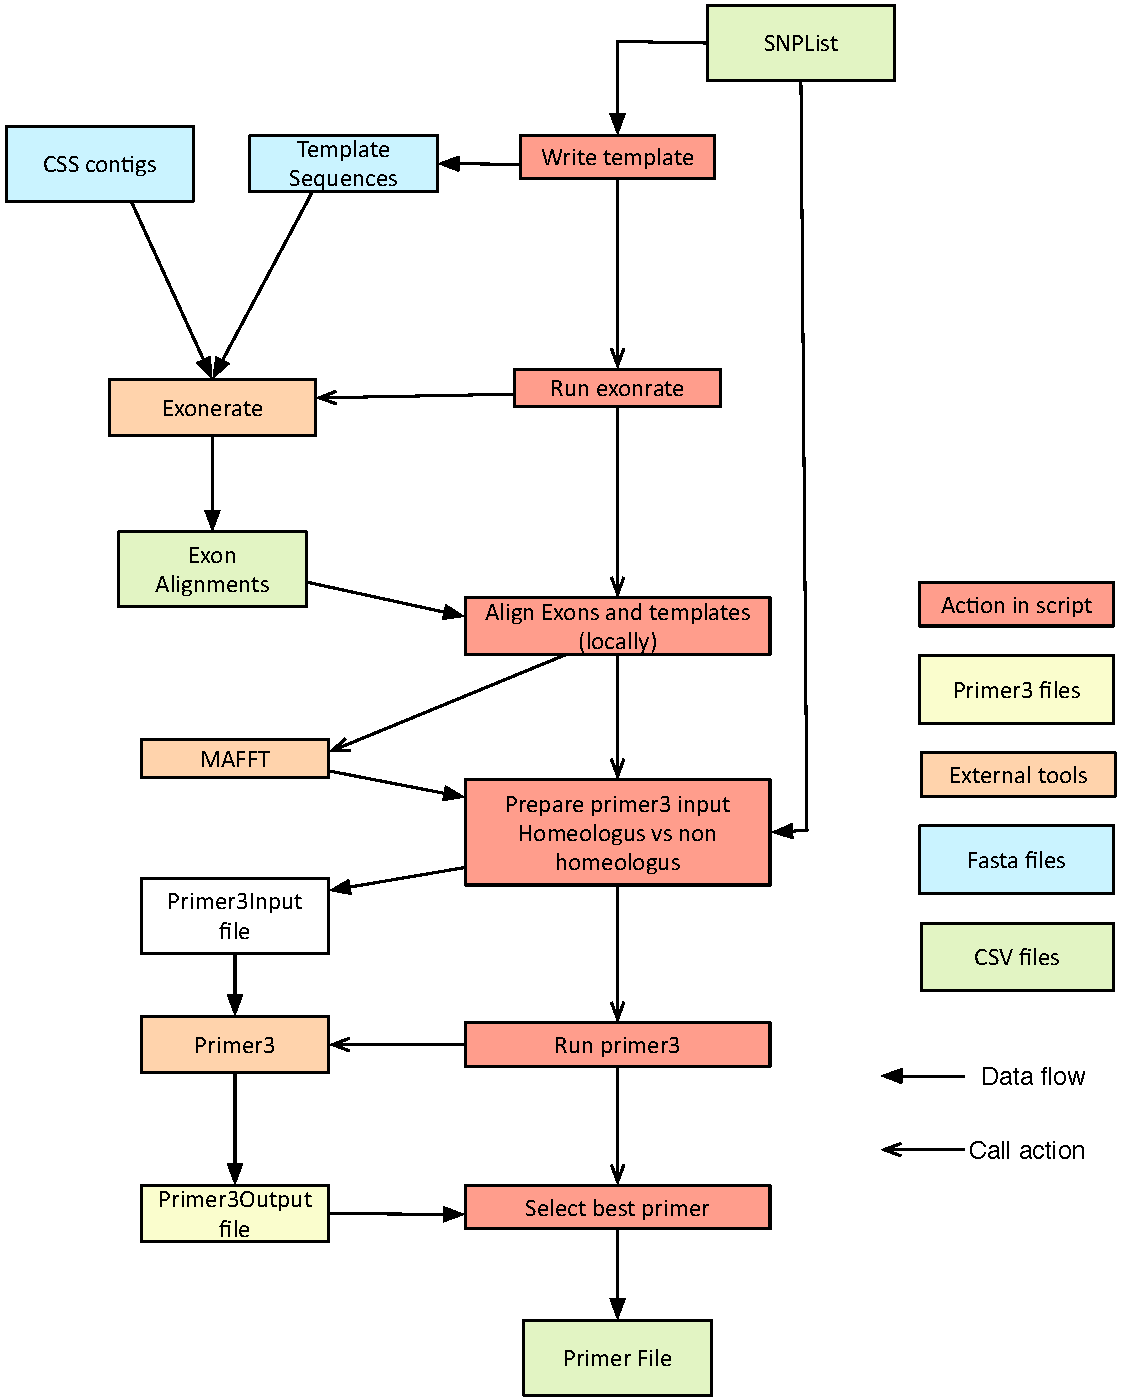
\includegraphics[width=1\textwidth]{PolyMarker/Figures/pipeline.pdf}
        \caption{Steps and tools called by PolyMarker. The colour of the boxes represent: the step is an action inside the script(red); actions of the script(orange); temporary files(yellow); inputs(blue) and; outpus(green)}
        \label{fig:poly:pipeline}
\end{figure}

The PolyMarker input consist on SNP list with: unique name for the marker, the target chromosome and the sequence for the marker. 
The alternative alleles are surrounded by square brackets within the sequence. PolyMarker can take a list of several markers and design them in batch (Figure \ref{fig:poly:input}). 
A \texttt{FASTA} file is produced with all the template sequences, with the alternative alleles substituted by the IUAPC ambiguity codes \citep{Cornish-Bowden1985}. 
The flanking sequence surrounding the SNP is limited by default to 100bp to reduce the search time and avoid missing regions that diverge near the SNP, as when the variation is near an intron-exon junction. 
%%TODO: Should we elaborate more here? 

The template sequences are searched in the reference sequence using \texttt{exonerate}\citep{Slater2005}, figure \ref{fig:poly:globalSearch}. 
The alignment is run with the \texttt{--model est2genome} option, to allow the search of sequences coming from transcripts, a common source of SNPs\citep{Allen2011}. 
The exonerate output is formatted with the \texttt{--ryo} (roll your own format) to get an output easy to parse. 
All the hits that contain the SNP are extracted from the reference with a flanking sequence that extend out of the hit, by defualt, to 100bp on each side of the SNP Figure \ref{fig:poly:globalAround}.
The size of the flanking sequence can be set to different sizes to allow the design of different types of primers. 
Different homoeologues may contain small indels (Figure \ref{fig:poly:globalSequence}). 
To enable a comparasion base-per-base, a local alignment with \texttt{MAFFT} \citep{Katoh2013} is produced (Figure \ref{fig:poly:localSequence}. 
For wheat, PolyMarker uses the contigs from \cite{Mayer2014}, as deposited in Ensembl. 
As new releases of the wheat genome are made available, different parsers to assign the chromosome to each sequence can be added with little effort to PolyMarker. 

%\section{Global alignment} 
%Search of the contigs with the sequence in the CSS reference and the importance of being able to distinguish between homoeologous regions. 


\begin{figure}
    \centering
    \begin{subfigure}[b]{0.8\textwidth}
        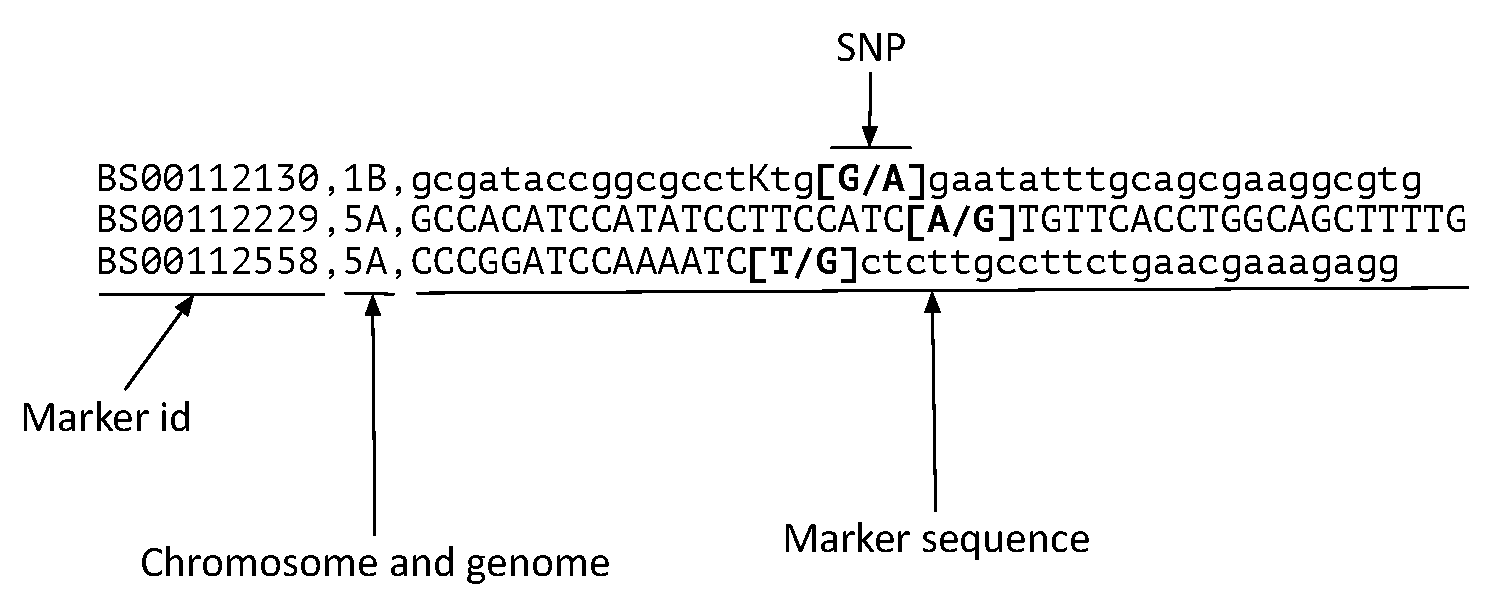
\includegraphics[width=1\textwidth]{PolyMarker/Figures/aln/input.pdf} 
        \caption{PolyMarker input. The alternative alleles are sorrounded by brackets.}
        \label{fig:poly:input}
    \end{subfigure}

    \begin{subfigure}[b]{0.4\textwidth}
        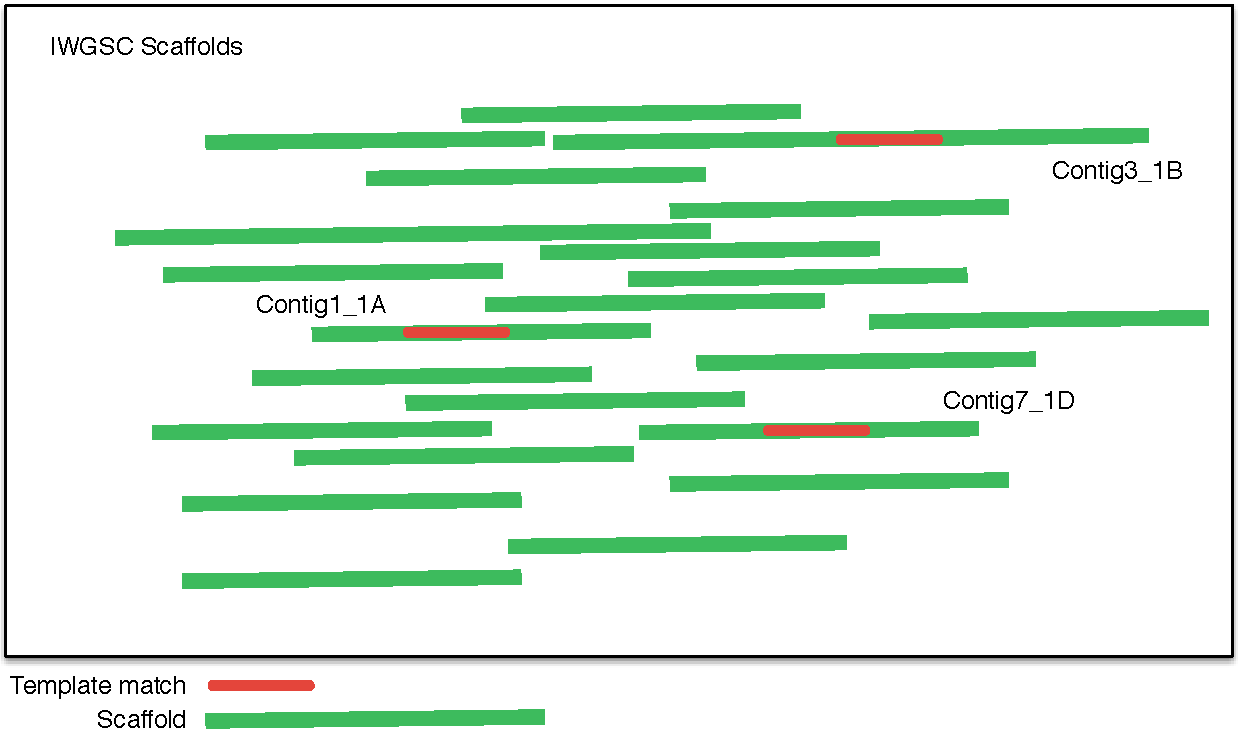
\includegraphics[width=1\textwidth]{PolyMarker/Figures/aln/scaffoldsSearch.pdf}
        \caption{Global search of templates in the reference contigs.}
        \label{fig:poly:globalSearch}
    \end{subfigure}
    ~ %add desired spacing between images, e. g. ~, \quad, \qquad, \hfill etc. 
      %(or a blank line to force the subfigure onto a new line)
    \begin{subfigure}[b]{0.4\textwidth}
        \raisebox{10mm} { 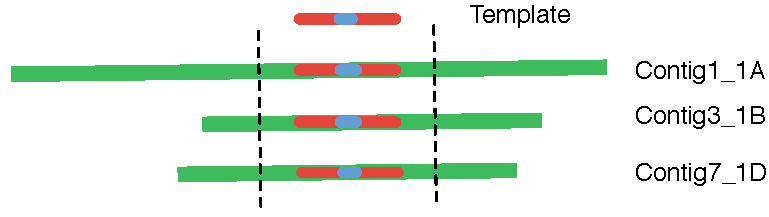
\includegraphics[width=1\textwidth]{PolyMarker/Figures/aln/scaffoldsFoundAround.pdf} }
        \caption{Selected regions around the SNP on every chromosome.}
        \label{fig:poly:globalAround} 
    \end{subfigure}
    
    \begin{subfigure}[b]{0.4\textwidth}
        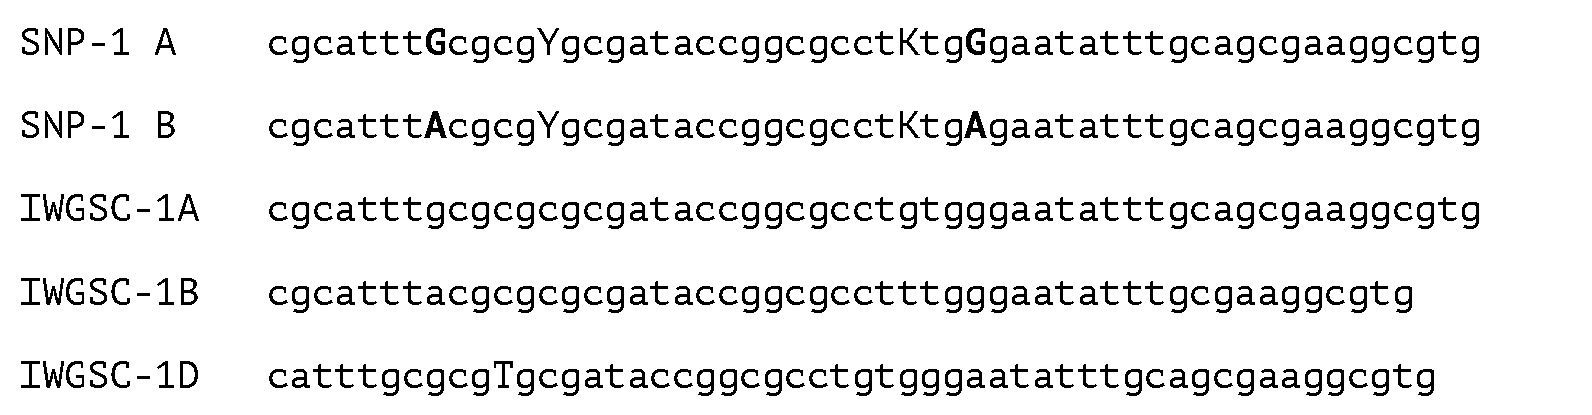
\includegraphics[width=1\textwidth]{PolyMarker/Figures/aln/scaffoldsFound.pdf}
        \caption{Sequence of found regions around the SNP.}
        \label{fig:poly:globalSequence}
    \end{subfigure}
    ~ %add desired spacing between images, e. g. ~, \quad, \qquad, \hfill etc. 
      %(or a blank line to force the subfigure onto a new line)
    \begin{subfigure}[b]{0.4\textwidth}
        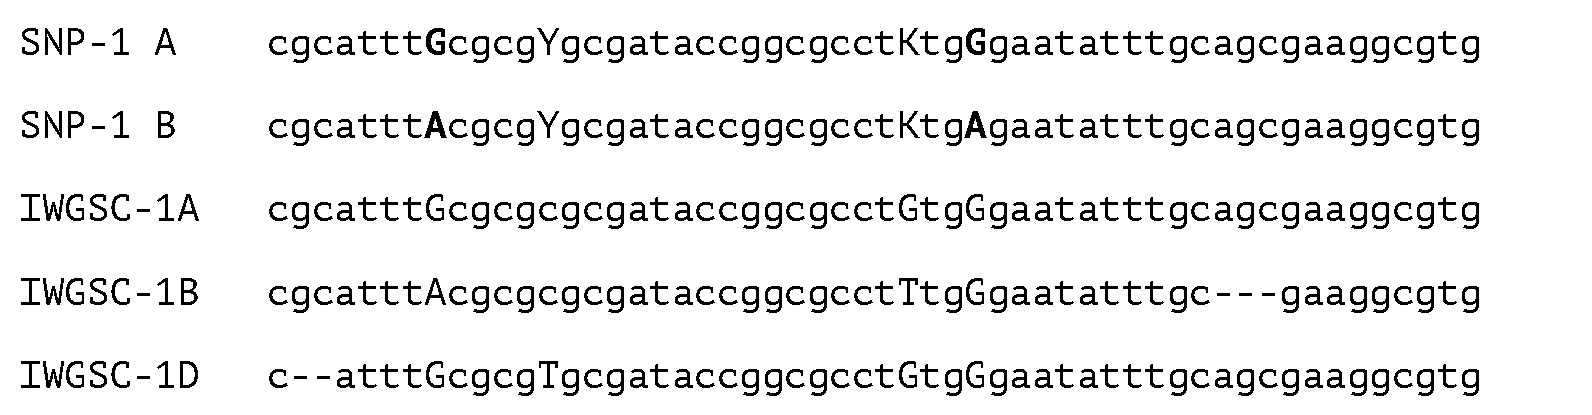
\includegraphics[width=1\textwidth]{PolyMarker/Figures/aln/localAlignment.pdf} 
        \caption{Local alignment on regions around the SNP detects indels.}
        \label{fig:poly:localSequence}
    \end{subfigure}

    \begin{subfigure}[b]{0.8\textwidth}
        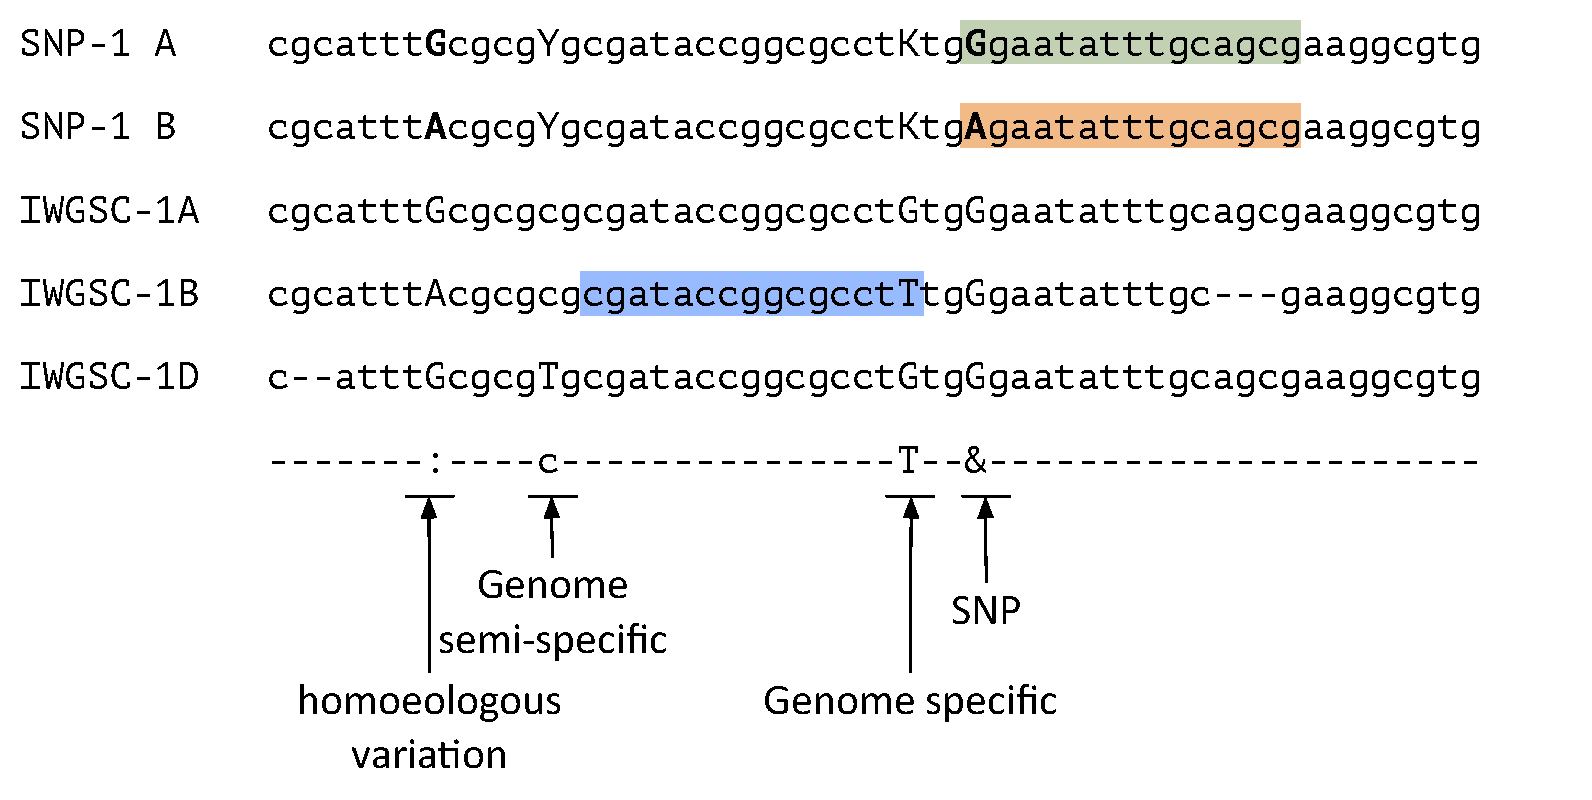
\includegraphics[width=1\textwidth]{PolyMarker/Figures/aln/mask.pdf} 
        \caption{Alignment with mask and primer candidates.}
        \label{fig:poly:mask}
    \end{subfigure}
    \caption{Alignments done by PolyMarker.}\label{fig:global}
\end{figure}

\section{Primer design tools} 
In this section, the principles of \textit{in silico} primer design are discussed, and why not simply selecting a genomic variation is enough (thermal stability, primers folding on themselves)

\section{Primer selection algorithms} 
Different algorithms to select the \"best primer\". 

\subsection{KASP markers} 
For KASP markers, the product should be as short as possible with the mutation in the first three bases. 

\section{Designed markers} Details of the generated primers for the 80k iSelect chip and the 820k axiom chip. This section also include counts on how many are genome specific, semi-specific and non specific. Also an analysis of how many are repeated or map to more than one chromosome perfectly.

\subsection{Regular markers}  
PolyMarker was designed for KASP assays, but it was later extended to produce regular primers, where both primers start with a genome-specific base. This simplifies the design of primers for regular PCR and capillary sequencing. 




\subsection{Deletion algorithms}
Algorithm to produce KASP for deletions in polyploids. 

\begin{figure}
    \centering
    \begin{subfigure}[b]{0.4\textwidth}
        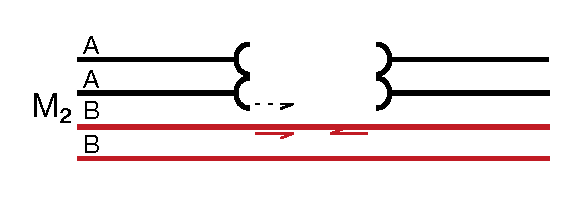
\includegraphics[width=1\textwidth]{PolyMarker/Figures/deletions/homM2.pdf}
        \caption{Homozygous deletion on $M_{2}$}
        \label{fig:poly:homM2}
    \end{subfigure}
    ~ %add desired spacing between images, e. g. ~, \quad, \qquad, \hfill etc. 
      %(or a blank line to force the subfigure onto a new line)
    \begin{subfigure}[b]{0.4\textwidth}
        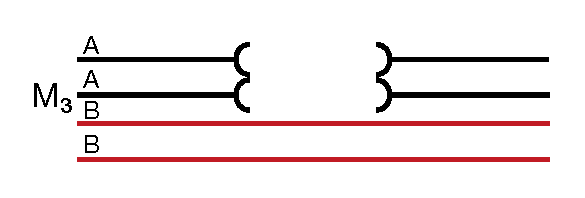
\includegraphics[width=1\textwidth]{PolyMarker/Figures/deletions/homM3.pdf} 
        \caption{Homozygous deletion on  $M_{3}$}
        \label{fig:poly:homM3}
    \end{subfigure}
    
    \begin{subfigure}[b]{0.3\textwidth}
        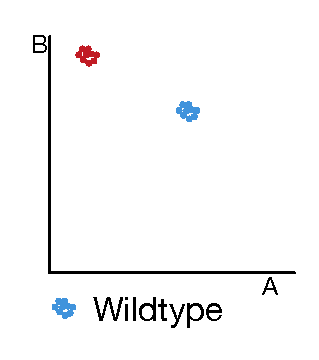
\includegraphics[width=1\textwidth]{PolyMarker/Figures/deletions/homReal.pdf}
        \caption{KASP amplification for a real deletion}
        \label{fig:poly:homReal}
    \end{subfigure}
    ~ %add desired spacing between images, e. g. ~, \quad, \qquad, \hfill etc. 
      %(or a blank line to force the subfigure onto a new line)
    \begin{subfigure}[b]{0.3\textwidth}
        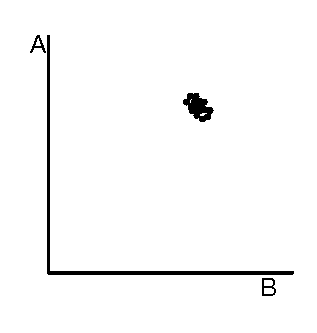
\includegraphics[width=1\textwidth]{PolyMarker/Figures/deletions/homFalse.pdf} 
        \caption{KASP amplification on false positive}
        \label{fig:poly:homFalse}
    \end{subfigure}
    \begin{subfigure}[b]{0.3\textwidth}
        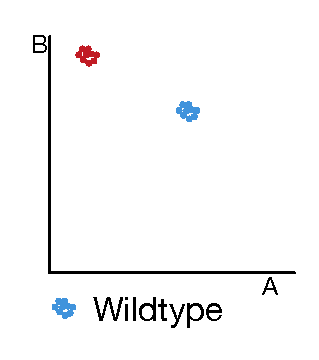
\includegraphics[width=1\textwidth]{PolyMarker/Figures/deletions/homReal.pdf} 
        \caption{Example of validated deletion on mutant poulation}
        \label{fig:poly:homTest}
    \end{subfigure}
    \caption{PolyMarker used to find primers to detect long deletions in tetraploid wheat.}
    \label{fig:poly:homDel}
\end{figure}



\section{Conclusions} Remarks on the importance of getting the primers right, and the time saved by automating the primer selection. Also mention other primer design tools that have been inspired by polymarker: \cite{Ma2015}, \cite{Wang2016}

PolyMarker has been used succesfully to design genome-specific primers in several projects. 


